\chapter{Sequential-Recognition-Engine}
\label{sequential}

Die bis hierher beschriebene Recognition-Engine erkennt Editieroperationen nur dann, wenn sie nicht
in sequentieller Abhängigkeit zueinander stehen. Sind zwei Editierregeln X und Y sequentiell
abhängig, dann bedeutet das, Editierregel Y kann erst angewandt werden, wenn Editierregel X bereits
ausgeführt wurde. In diesem Fall würde also nur die Editieroperationen der Editierregel X durch die
entsprechende Erkennungsregel in der Differenz geliftet. Es können auch mehrere Editierregeln in
sequentieller Abhängigkeit stehen. Grundsätzlich lassen sich zwei Arten von Abhängigkeiten
unterscheiden.

\begin{itemize}
  \item \textbf{Create-Use-Dependence:} Eine solche Abhängigkeit tritt immer dann auf, wenn ein
  neu hinzugefügtes Objekt wieder als Kontext für eine weitere Editieroperation benötigt wird. Der
  Kontext ist im Fall einer Henshin Editierregel immer der \texttt{<<preserve>>} Teil der Regel. Am
  häufigsten wird der Container eines hinzuzufügenden oder zu entfernenden Objekts als Kontext
  benötigt.
  
  \begin{figure}[htbp]
    \centering
    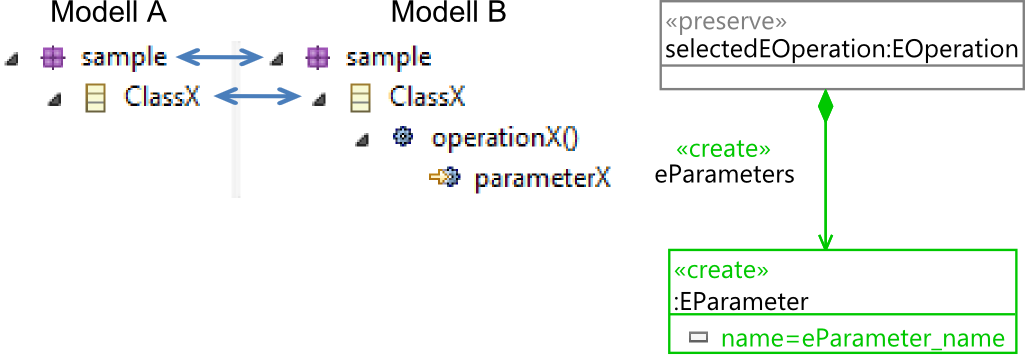
\includegraphics[scale=1.4]{images/create-use-dependence.png}
    \caption{Create-Use-Dependence Beispiel}
    \label{fig:create-use-dependence}
  \end{figure}
  
  Abbildung \ref{fig:create-use-dependence} beschreibt einen solchen Fall. Hier existiert eine
  Korrespondenz zwischen dem Paket \texttt{sample} und der Klasse \texttt{ClassX}. Die Operation
  \texttt{operationX()} und der Parameter \texttt{parameterX} wurden dem Modell hinzugefügt. Das
  Einfügen der Operation kann zunächst problemlos durch die entsprechende Erkennungsregel geliftet
  werden. Wie in der Abbildung \ref{fig:create-use-dependence} der Editierregel zum einfügen eines
  Parameters zu erkennen ist, wird hier eine bereits bestehende \texttt{EOperation} als Kontext
  erwartet. Innerhalb der Erkennungsregel ergibt sich nun das Problem, dass für die
  \texttt{EOperation} nach einem Correspondence-Pattern gesucht wird. Es existiert aber nur ein
  Add-Object-Pattern für \texttt{operationX()}. Daher wird das einfügen des Parameters  
  \texttt{parameterX} nicht geliftet.
  
  %Der Parameter Typ wurde aus Platzgründen weggelassen.

\item \textbf{Removed-Used-Dependence:} Das Problem dieser Abhängigkeit verhält sich im Prinzip
analog zum Create-Use-Dependence Problem. In diesem Fall wurde der Kontext, auf den sich die
erste Editieroperation bezog, im nächsten Schritt durch eine weitere Editieroperation entfernt.
Damit ergibt sich beim Lifting grundsätzlich das gleiche Problem.

Wie Abbildung \ref{fig:removed-used-dependence} zeigt, fehlt wieder die Korrespondenz
für \texttt{operationX()}, um das Entfernen des Parameters \texttt{parameterX} zu liften, da für
\texttt{operationX()} nur ein Remove-Object-Pattern in der Differenz existiert. 

  \begin{figure}[htbp]
    \centering
    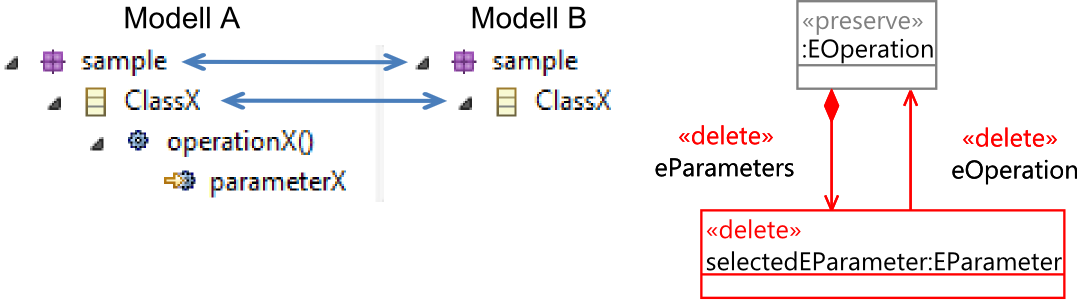
\includegraphics[scale=1.4]{images/removed-used-dependence.png}
    \caption{Removed-Used-Dependence Beispiel}
    \label{fig:removed-used-dependence}
  \end{figure}

\end{itemize}
Eine Möglichkeit dieses Problem zu betrachten ist es davon auszugehen, dass für ein vollständiges
Lifting immer alle Zwischenzustände des Modells benötigt werden, bevor eine Create-Use- oder
Removed-Used-Dependence entsteht. Die vollständig geliftete Differenz wäre dann die Summe aller
gelifteten Zwischenzustände. Genau dieses Prinzip wird von der Sequential-Recognition-Engine
verfolgt. Die Hauptaufgabe besteht darin die erwähnten Zwischenzustände zu berechnen. Das Lifting
zwischen zwei Modell Zuständen wird wie bisher von der Recognition-Engine mit nachfolgendem
Post-Processing übernommen.

Die Zwischenzustände errechnen sich immer aus dem gelifteten Teil der Differenz. Startet die 
Sequential-Recognition-Engine also mit einer ungelifteten Differenz, wird zunächst die normale
Recognition-Engine aufgerufen, um danach alle Semantic-Change-Sets durch das Post-Processing
überschneidungsfrei zu machen. Die Überschneidungsfreiheit ist insofern wichtig, damit die folgenden
Schritte nicht mehrfach ausgeführt werden. Als nächstes werden alle low-level Änderungen, welche
durch Semantic-Change-Sets gruppiert sind, auf die Modelle angewendet um die Zwischenzustände zu
erzeugen:

\begin{enumerate}
  \item Als erstes werden low-level Änderungen vom Typ Add-Object behandelt. Ein Add-Object
  referenziert immer ein Objekt (\texttt{objB}) aus Modell B. Von diesem Objekt wird nun eine Kopie
  erstellt (\texttt{objA}). Als nächstes wird die entsprechende Correspondence zwischen
  \texttt{objA} und \texttt{objB} angelegt und der Differenz hinzugefügt. Es ist zu beachten, dass 
  \texttt{objA} zu diesem Zeitpunkt nur durch die Correspondence referenziert wird, es wird hier
  noch kein Container Objekt festgelegt. Die Container Referenzen werden wie normale Referenzen erst
  nach Anlegen aller Objekte eingefügt. Das hat den Vorteil, dass keine Abhängigkeiten zwischen
  Objekten beachtet werden müssen, die innerhalb eines Semantic-Change-Sets auftreten können.
 
  \item Die Add-References werden jetzt ebenfalls in Modell A eingefügt. Dazu muss zunächst
  Quelle und Ziel der einzufügenden Referenz aus Modell B auf Modell A abgebildet werden. Dazu
  werden die Correspondences zwischen den Quell- und Zielobjekten der beiden Modelle verwendet. Als
  nächstes wird dann die Referenz des Modell A Quellobjekts auf das entsprechende Modell A
  Zielobjekt gesetzt.
  
  \item Die referenzierten Objekte der Remove-Object low-level Änderungen werden analog zu den
  der Add-Objekts kopiert und als Modell B Objekt in einer neuen Correspondence abgelegt.
 
  \item Alle Remove-References werden ebenfalls analog zu den Add-References von Modell A auf
  Modell B übertragen.
  
  \item Für alle Attribute-Value-Changes werden die Werte der Attribute in Modell A auf die neuen
  Werte aus Modell B gesetzt. Dies reicht in der Regel aus, um Attribute zwischen Modell A und
  Modell B in der Erkennungsregel auf Gleichheit zu prüfen. (siehe \ref{avc-preserve}
  Preserved-Attribute-Value-Pattern)
\end{enumerate}
Nachdem alle low-level Änderungen aus allen Semantic-Change-Sets mit den Modellen verschmolzen
wurden, können sowohl die low-level Änderungen als auch die Semantic-Change-Sets temporär aus der
Differenz entfernt werden. Der so errechnete Zwischenzustand dient nun als Ausgangspunkt für das
nächste Lifting und Post-Processing. Dieser Vorgang wird solange wiederholt, wie in einem Durchlauf
noch neue Semantic-Change-Sets erzeugt werden oder bis keine low-level Änderungen mehr in der
Differenz vorhanden sind. 

Durch die in Abschnitt \ref{filter} beschriebene Filterung der Regeln reduziert sich die Anzahl der
Erkennungsregeln von Schritt zu Schritt, da immer weniger low-level Änderungen in der Differenz
zurück bleiben. Würde man die Editierregeln auf ihre Abhängigkeit analysieren, dann könnte man die
anzuwendenden Erkennungsregeln noch gezielter eingrenzen. Zunächst würde ein ganz normaler
Erkennungsdurchlauf erfolgen. In den nächsten Schritten würden dann immer nur die Erkennungsregeln
angewendet, welche mindestens eine sequentielle Abhängigkeit zu den Editieroperationen haben, die im
Schritt zuvor erkannt wurden.

Am Ende werden alle Semantic-Change-Sets, inklusive deren low-level Änderungen, die in den einzelnen
Lifting-Schritten entfernt wurden, wieder in der Differenz zusammengeführt. Außerdem müssen alle
eingefügten Correspondences wieder entfernt werden, um die Differenz auf ihren Ausgangspunkt
zurückzusetzen.

%\subsubsection{Sequential-Lifting-Beispiel}